\documentclass{article}

\usepackage{tikz} 
\usetikzlibrary{automata, positioning, arrows} 

\usepackage{amsthm}
\usepackage{amsfonts}
\usepackage{amsmath}
\usepackage{amssymb}
\usepackage{fullpage}
\usepackage{color}
\usepackage{parskip}
\usepackage{hyperref}
\usepackage{graphicx}

  \hypersetup{
    colorlinks = true,
    urlcolor = blue,
    linkcolor= blue,
    citecolor= blue,
    filecolor= blue,
    }
    
\usepackage{listings}
\usepackage[utf8]{inputenc}                                                    
\usepackage[T1]{fontenc}      
\usepackage{enumitem}                                                 

\definecolor{dkgreen}{rgb}{0,0.6,0}
\definecolor{gray}{rgb}{0.5,0.5,0.5}
\definecolor{mauve}{rgb}{0.58,0,0.82}

\lstset{frame=tb,
  language=haskell,
  aboveskip=3mm,
  belowskip=3mm,
  showstringspaces=false,
  columns=flexible,
  basicstyle={\small\ttfamily},
  numbers=none,
  numberstyle=\tiny\color{gray},
  keywordstyle=\color{blue},
  commentstyle=\color{dkgreen},
  stringstyle=\color{mauve},
  breaklines=true,
  breakatwhitespace=true,
  tabsize=3
}

\newtheoremstyle{theorem}
  {\topsep} {\topsep} {\itshape\/} {0pt} {\bfseries} {.} {5pt plus 1pt minus 1pt} {}
\theoremstyle{theorem} 
   \newtheorem{theorem}{Theorem}[section]
   \newtheorem{corollary}[theorem]{Corollary}
   \newtheorem{lemma}[theorem]{Lemma}
   \newtheorem{proposition}[theorem]{Proposition}
\theoremstyle{definition}
   \newtheorem{definition}[theorem]{Definition}
   \newtheorem{example}[theorem]{Example}
\theoremstyle{remark}    
  \newtheorem{remark}[theorem]{Remark}

\lstdefinelanguage{PythonDFARun}{
    keywords={def, for, in, if, return},
    keywordstyle=\color{blue}\bfseries,
    morekeywords={self},
    keywordstyle=[2]\color{purple},
    morekeywords=[2]{self},
    stringstyle=\color{red},
    commentstyle=\color{gray},
    identifierstyle=\color{black},
    sensitive=true
}

\lstset{
    language=PythonDFARun,
    basicstyle=\ttfamily\footnotesize,
    frame=single,
    showstringspaces=false,
    tabsize=4
}

\title{CPSC-354 Report}
\author{Jeffrey Bok  \\ Chapman University}
\date{\today} 

\begin{document}

\maketitle

\begin{abstract}
This report documents my exploration of programming language theory through CPSC-354. It covers foundational topics including abstract reduction systems, lambda calculus, formal proofs in Lean, and the Curry-Howard correspondence. The synthesis section connects these concepts to reveal computation as systematic rewriting according to formal rules. Through weekly homework and supplementary materials, I developed an understanding of how mathematical principles underlie modern programming languages.

\end{abstract}

\setcounter{tocdepth}{3}
\tableofcontents

\section{Introduction}\label{intro}

This report chronicles my journey through CPSC-354: Programming Languages, documenting both the technical work completed each week and the conceptual understanding developed throughout the semester. The course explored fundamental questions about computation: What makes a programming language? How can we prove programs correct? What are the mathematical foundations underlying all of computation?

The report is organized as follows: Section 2 presents weekly homework solutions with exploration and discussion questions; Section 3 synthesizes the major themes connecting all topics; Section 4 documents engagement with supplementary materials; and Section 5 provides critical reflection on the course's place in software engineering education.

\section{Week by Week}\label{homework}

\subsection{Week 1}
\subsubsection{Homework}

What is the MU Puzzle and how do you "solve" it?:

The MU puzzle is a logic puzzle created by Douglas Hofstadter in his 1979 book "Gödel, Escher, Bach: An Eternal Golden Braid." It's designed to illustrate concepts about formal systems, computability, and the limits of rule-based reasoning. The rules are below:

Rule I: If a string ends in I, you can add U to the end (xI → xIU)\newline
Rule II: If you have Mx, you can make Mxx (double everything after M)\newline
Rule III: If you find III anywhere in your string, you can replace it with U (xIIIy → xUy)\newline
Rule IV: If you find UU anywhere in your string, you can remove it (xUUy → xy)

To "solve" the puzzle, you try to apply a combination of rules step by step, creating new strings. 
Eventually, you'll find that MU can never be reached because the rules never allow you to remove the odd number of \texttt{I}'s needed to get zero. 

\subsubsection{Exploration}
Hofstadter used this puzzle to demonstrate how formal systems can have inherent limitations - some statements that seem like they should be provable within a system are actually unprovable. This connects to Gödel's incompleteness theorems and fundamental questions about the nature of mathematical truth and computation.

Programming languages are formal systems, just like the MU puzzle. They have:

\begin{itemize}
\item Syntax rules (what constitutes valid code)
\item Transformation rules (how expressions evaluate)  
\item Semantic constraints (what programs can actually compute)
\end{itemize}

The MU puzzle demonstrates that even simple rule sets can have hidden limitations - similarly, programming languages have inherent computational boundaries.

\subsubsection{Questions}
1. The impossibility of reaching "MU" from "MI" is provable, yet someone working within the system might not realize this. How does this relate to the halting problem and undecidable questions in programming?

\subsection{Week 2}
\subsubsection{Homework}
    Consider the following list of ARSs:\newline
    \begin{enumerate}
    \item $A = \{\}$.
    \item $A = \{a\}$ and $R = \{\}$.
    \item $A = \{a\}$ and $R = \{(a,a)\}$.
    \item $A = \{a,b,c\}$ and $R = \{(a,b),(a,c)\}$.
    \item $A = \{a,b\}$ and $R = \{(a,a),(a,b)\}$.
    \item $A = \{a,b,c\}$ and $R = \{(a,b),(b,b),(a,c)\}$.
    \item $A = \{a,b,c\}$ and $R = \{(a,b),(b,b),(a,c),(c,c)\}$.
    \end{enumerate}
    
    Draw a picture for each of the ARSs above. Are the ARSs terminating? Are they confluent? Do they have unique normal forms?

    Try to find an example of an ARS for each of the possible 8 combinations. Draw pictures of these examples.

        
    \paragraph{ARS 1: $A = \{\}$}
    \begin{center}
    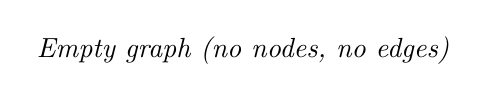
\begin{tikzpicture}
        \node at (0,0) {\textit{Empty graph (no nodes, no edges)}};
    \end{tikzpicture}
    \end{center}
    \textbf{Terminating:} YES \quad \textbf{Confluent:} YES \quad \textbf{Unique Normal Forms:} YES
    
    \paragraph{ARS 2: $A = \{a\}$, $R = \{\}$}
    \begin{center}
    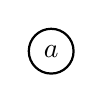
\begin{tikzpicture}[node distance=2cm, auto, thick]
        \node[circle, draw] (a) {$a$};
    \end{tikzpicture}
    \end{center}
    \textbf{Terminating:} YES \quad \textbf{Confluent:} YES \quad \textbf{Unique Normal Forms:} YES
    
    \paragraph{ARS 3: $A = \{a\}$, $R = \{(a,a)\}$}
    \begin{center}
    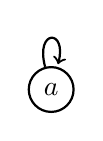
\begin{tikzpicture}[node distance=2cm, auto, thick, -latex]
        \node[circle, draw] (a) {$a$};
        \path (a) edge[loop above] (a);
    \end{tikzpicture}
    \end{center}
    \textbf{Terminating:} NO \quad \textbf{Confluent:} YES \quad \textbf{Unique Normal Forms:} NO
    
    \paragraph{ARS 4: $A = \{a,b,c\}$, $R = \{(a,b),(a,c)\}$}
    \begin{center}
    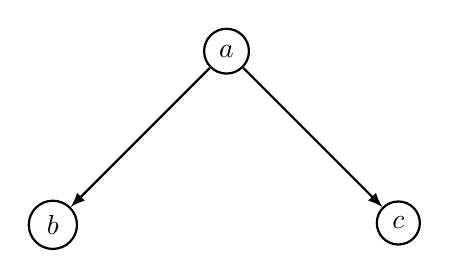
\begin{tikzpicture}[node distance=2.5cm, auto, thick, -latex]
        \node[circle, draw] (a) {$a$};
        \node[circle, draw] (b) [below left=of a] {$b$};
        \node[circle, draw] (c) [below right=of a] {$c$};
        
        \path (a) edge (b);
        \path (a) edge (c);
    \end{tikzpicture}
    \end{center}
    \textbf{Terminating:} YES \quad \textbf{Confluent:} NO \quad \textbf{Unique Normal Forms:} NO
    
    \paragraph{ARS 5: $A = \{a,b\}$, $R = \{(a,a),(a,b)\}$}
    \begin{center}
    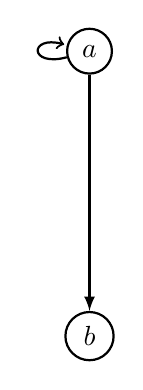
\begin{tikzpicture}[node distance=3cm, auto, thick, -latex]
        \node[circle, draw] (a) {$a$};
        \node[circle, draw] (b) [below=of a] {$b$};
        
        \path (a) edge[loop left] (a);
        \path (a) edge (b);
    \end{tikzpicture}
    \end{center}
    \textbf{Terminating:} NO \quad \textbf{Confluent:} NO \quad \textbf{Unique Normal Forms:} NO
    
    \paragraph{ARS 6: $A = \{a,b,c\}$, $R = \{(a,b),(b,b),(a,c)\}$}
    \begin{center}
    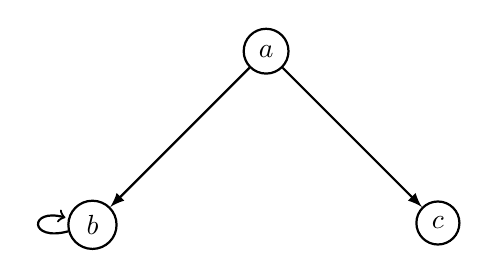
\begin{tikzpicture}[node distance=2.5cm, auto, thick, -latex]
        \node[circle, draw] (a) {$a$};
        \node[circle, draw] (b) [below left=of a] {$b$};
        \node[circle, draw] (c) [below right=of a] {$c$};
        
        \path (a) edge (b);
        \path (a) edge (c);
        \path (b) edge[loop left] (b);
    \end{tikzpicture}
    \end{center}
    \textbf{Terminating:} NO \quad \textbf{Confluent:} NO \quad \textbf{Unique Normal Forms:} NO
    
    \paragraph{ARS 7: $A = \{a,b,c\}$, $R = \{(a,b),(b,b),(a,c),(c,c)\}$}
    \begin{center}
    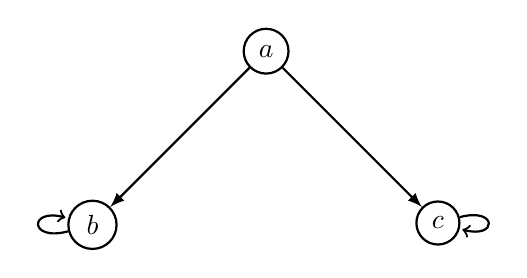
\begin{tikzpicture}[node distance=2.5cm, auto, thick, -latex]
        \node[circle, draw] (a) {$a$};
        \node[circle, draw] (b) [below left=of a] {$b$};
        \node[circle, draw] (c) [below right=of a] {$c$};
        
        \path (a) edge (b);
        \path (a) edge (c);
        \path (b) edge[loop left] (b);
        \path (c) edge[loop right] (c);
    \end{tikzpicture}
    \end{center}
    \textbf{Terminating:} NO \quad \textbf{Confluent:} NO \quad \textbf{Unique Normal Forms:} NO

    \paragraph{8 Combinations Table}
    \begin{center}
        \begin{tabular}{|c|c|c|l|}
        \hline
        \textbf{Confluent} & \textbf{Terminating} & \textbf{Unique NF} & \textbf{Example} \\
        \hline
        True & True & True & $A = \{a\}$, $R = \{\}$ \\
        True & True & False & $A = \{\}$, $R = \{\}$ \\
        True & False & True & $A = \{a,b\}$, $R = \{(a,b),(b,b)\}$ \\
        True & False & False & $A = \{a\}$, $R = \{(a,a)\}$ \\
        False & True & True & $A = \{a,b,c,d\}$, $R = \{(a,b),(a,c),(c,d)\}$ \\
        False & True & False & $A = \{a,b,c\}$, $R = \{(a,b),(a,c)\}$ \\
        False & False & True & $A = \{a,b,c\}$, $R = \{(a,b),(b,a),(a,c),(c,a)\}$ \\
        False & False & False & $A = \{a,b,c\}$, $R = \{(a,b),(b,b),(a,c)\}$ \\
        \hline
        \end{tabular}
    \end{center}

    \paragraph{Examples for 8 Combinations}

    \subparagraph{Example 1: Confluent=T, Terminating=T, Unique Normal Forms=T}
    $A = \{a\}$, $R = \{\}$
    \begin{center}
    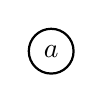
\begin{tikzpicture}[node distance=2cm, auto, thick]
        \node[circle, draw] (a) {$a$};
    \end{tikzpicture}
    \end{center}

    \subparagraph{Example 2: Confluent=T, Terminating=T, Unique Normal Forms=F}
    $A = \{\}$, $R = \{\}$
    \begin{center}
    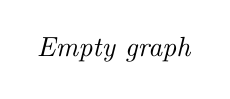
\begin{tikzpicture}
        \node at (0,0) {\textit{Empty graph}};
    \end{tikzpicture}
    \end{center}

    \subparagraph{Example 3: Confluent=T, Terminating=F, Unique Normal Forms=T}
    $A = \{a,b\}$, $R = \{(a,b),(b,b)\}$
    \begin{center}
    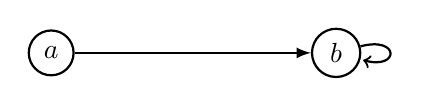
\begin{tikzpicture}[node distance=3cm, auto, thick, -latex]
        \node[circle, draw] (a) {$a$};
        \node[circle, draw] (b) [right=of a] {$b$};
        
        \path (a) edge (b);
        \path (b) edge[loop right] (b);
    \end{tikzpicture}
    \end{center}

    \subparagraph{Example 4: Confluent=T, Terminating=F, Unique Normal Forms=F}
    $A = \{a\}$, $R = \{(a,a)\}$
    \begin{center}
    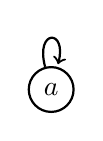
\begin{tikzpicture}[node distance=2cm, auto, thick, -latex]
        \node[circle, draw] (a) {$a$};
        \path (a) edge[loop above] (a);
    \end{tikzpicture}
    \end{center}

    \subparagraph{Example 5: Confluent=F, Terminating=T, Unique Normal Forms=T}
    $A = \{a,b,c,d\}$, $R = \{(a,b),(a,c),(c,d)\}$
    \begin{center}
        \begin{tikzpicture}[node distance=2.5cm, auto, thick, -latex]
            \node[circle, draw] (a) {$a$};
            \node[circle, draw] (b) [below left=of a] {$b$};
            \node[circle, draw] (c) [below right=of a] {$c$};
            \node[circle, draw] (d) [below=of c] {$d$};
            
            \path (a) edge (b);
            \path (a) edge (c);
            \path (c) edge (d);
        \end{tikzpicture}
    \end{center}

    \subparagraph{Example 6: Confluent=F, Terminating=T, Unique Normal Forms=F}
    $A = \{a,b,c\}$, $R = \{(a,b),(a,c)\}$
    \begin{center}
        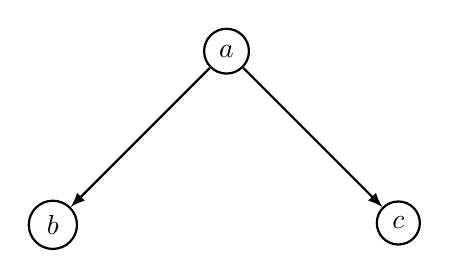
\begin{tikzpicture}[node distance=2.5cm, auto, thick, -latex]
            \node[circle, draw] (a) {$a$};
            \node[circle, draw] (b) [below left=of a] {$b$};
            \node[circle, draw] (c) [below right=of a] {$c$};
            
            \path (a) edge (b);
            \path (a) edge (c);
        \end{tikzpicture}
    \end{center}

    \subparagraph{Example 7: Confluent=F, Terminating=F, Unique Normal Forms=T}
    $A = \{a,b,c\}$, $R = \{(a,b),(b,a),(a,c),(c,a)\}$
    \begin{center}
    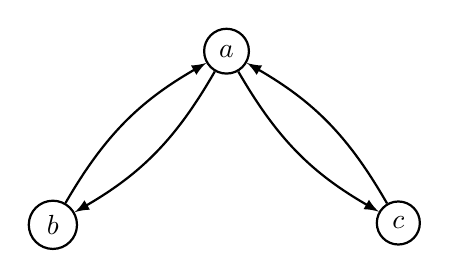
\begin{tikzpicture}[node distance=2.5cm, auto, thick, -latex]
        \node[circle, draw] (a) {$a$};
        \node[circle, draw] (b) [below left=of a] {$b$};
        \node[circle, draw] (c) [below right=of a] {$c$};
        
        \path (a) edge[bend left=15] (b);
        \path (b) edge[bend left=15] (a);
        \path (a) edge[bend right=15] (c);
        \path (c) edge[bend right=15] (a);
    \end{tikzpicture}
    \end{center}

    \subparagraph{Example 8: Confluent=F, Terminating=F, Unique Normal Forms=F}
    $A = \{a,b,c\}$, $R = \{(a,b),(b,b),(a,c)\}$
    \begin{center}
    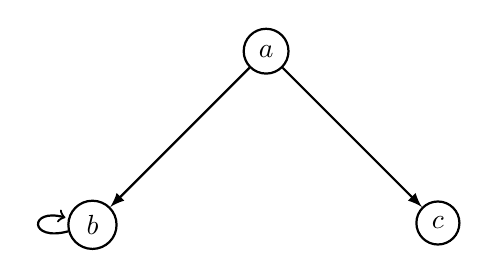
\begin{tikzpicture}[node distance=2.5cm, auto, thick, -latex]
        \node[circle, draw] (a) {$a$};
        \node[circle, draw] (b) [below left=of a] {$b$};
        \node[circle, draw] (c) [below right=of a] {$c$};
        
        \path (a) edge (b);
        \path (a) edge (c);
        \path (b) edge[loop left] (b);
    \end{tikzpicture}
    \end{center}

    \subsubsection{Exploration}
    Abstract Reduction Systems provide a mathematical foundation for understanding computation and rewriting. The properties of termination, confluence, and unique normal forms are fundamental to understanding how programming languages behave:
    
    \begin{itemize}
    \item \textbf{Termination} ensures that computations eventually halt
    \item \textbf{Confluence} guarantees that the order of operations doesn't affect the final result
    \item \textbf{Unique Normal Forms} means every expression has a single, well-defined simplified form
    \end{itemize}
    
    These concepts directly apply to programming language design, where we want predictable evaluation strategies and guaranteed termination for certain classes of programs.
    
    \subsubsection{Questions}
    1. How do the termination properties of ARSs relate to the halting problem in computation?\newline
    2. Why might a programming language designer prefer confluent systems over non-confluent ones?\newline

\subsection{Week 3}
\subsubsection{Homework}
Consider the rewrite rules:
\begin{itemize}
\item ab $\to$ ba
\item ba $\to$ ab  
\item aa $\to$ (empty string)
\item b $\to$ (empty string)
\end{itemize}

\subsubsection{Sample Reductions}
\textbf{Reducing abba:}

abba $\to$ baba (using ab $\to$ ba)

baba $\to$ bbaa (using ab $\to$ ba)

bbaa $\to$ baa (using b $\to$ empty)

baa $\to$ aa (using b $\to$ empty)

aa $\to$ empty (using aa $\to$ empty)

\textbf{Reducing bababa:}

bababa $\to$ bbaaaba (using ab $\to$ ba twice)

bbaaaba $\to$ baaaba (using b $\to$ empty)

baaaba $\to$ aaaba (using b $\to$ empty)

aaaba $\to$ aba (using aa $\to$ empty)

aba $\to$ baa (using ab $\to$ ba)

baa $\to$ aa (using b $\to$ empty)

aa $\to$ empty (using aa $\to$ empty)

\subsubsection{Analysis}
\textbf{Why is the ARS not terminating?}

The first two rules ab $\to$ ba and ba $\to$ ab create cycles. You can apply these rules forever, going back and forth between ab and ba.

\textbf{Find two strings that are not equivalent. How many non-equivalent strings can you find?}

Two strings that are not equivalent: "a" and "empty string". The string "a" cannot be reduced further, while other strings can reduce to empty.

\textbf{Equivalence classes and normal forms:}
There are exactly 2 equivalence classes:
\begin{enumerate}
\item Strings that reduce to empty string
\item Strings that reduce to "a"
\end{enumerate}

The normal forms are: empty string and "a"

\textbf{Modified terminating ARS:}
To make it terminating, always eliminate b's first, then eliminate aa's, then do swapping only if needed.

\textbf{Questions about strings that can be answered using the ARS:}
\begin{enumerate}
\item "Given a string, does it contain an even number of a's?"
\item "Given a string, does it contain an odd number of a's?"
\item "Are two strings equivalent under this rewrite system?"
\end{enumerate}

\subsection{Exercise 5b}
\subsubsection{Modified Rewrite Rules}
Same as Exercise 5, but change aa $\to$ empty to aa $\to$ a:
\begin{itemize}
\item ab $\to$ ba
\item ba $\to$ ab  
\item aa $\to$ a (pairs of a become single a)
\item b $\to$ (empty string)
\end{itemize}

\subsubsection{Sample Reductions}
\textbf{Reducing abba:}

abba $\to$ baba (using ab $\to$ ba)

baba $\to$ bbaa (using ab $\to$ ba)

bbaa $\to$ baa (using b $\to$ empty)

baa $\to$ aa (using b $\to$ empty)

aa $\to$ a (using aa $\to$ a)

\textbf{Reducing bababa:}

bababa $\to$ bbaaaba (using ab $\to$ ba twice)

bbaaaba $\to$ baaaba (using b $\to$ empty)

baaaba $\to$ aaaba (using b $\to$ empty)

aaaba $\to$ aaba (using aa $\to$ a)

aaba $\to$ abaa (using ab $\to$ ba)

abaa $\to$ baaa (using ab $\to$ ba)

baaa $\to$ aaa (using b $\to$ empty)

aaa $\to$ aa (using aa $\to$ a)

aa $\to$ a (using aa $\to$ a)

\subsubsection{Analysis}
\textbf{Why the ARS is not terminating:}
Same as Exercise 5 - the rules ab $\to$ ba and ba $\to$ ab create infinite cycles.

\textbf{Non-equivalent strings:}
Two strings that are not equivalent: "a" and "empty string". We can find exactly 2 non-equivalent strings.

\textbf{Equivalence classes and normal forms:}
There are exactly 2 equivalence classes:
\begin{enumerate}
\item Strings with even number of a's $\to$ reduce to empty
\item Strings with odd number of a's $\to$ reduce to "a"
\end{enumerate}

The normal forms are: empty string and "a"

\textbf{Modified terminating ARS:}
To make it terminating, use the same priority as Exercise 5:
\begin{enumerate}
\item b $\to$ empty (eliminate all b's first)
\item aa $\to$ a (reduce pairs of a's)
\item ab $\to$ ba (only if needed)
\end{enumerate}

\textbf{Questions about strings that can be answered using the ARS:}
\begin{enumerate}
\item "Given a string, does it contain an even number of a's?"
\item "Given a string, does it contain an odd number of a's?"
\item "Are two strings equivalent under this rewrite system?"
\end{enumerate}

\subsubsection{Exploration}
\subsubsection{Questions}
\begin{enumerate}
\item If two completely different sets of rewrite rules (Exercise 5 vs 5b) produce the same equivalence classes, what does this tell us about the relationship between implementation and specification in computer science?

\item If "abab" and "bbaa" are equivalent under this system, but clearly different as strings, what does "equivalence" really mean? Is mathematical equivalence different from everyday sameness?

\end{enumerate}

\subsection{Week 4}
\subsubsection{Homework}

\textbf{HW 4.1: Euclidean Algorithm Termination}

Consider the Euclidean algorithm for computing GCD:
\begin{lstlisting}[language=Python]
while b != 0:
    temp = b
    b = a mod b
    a = temp
return a
\end{lstlisting}

\paragraph{Conditions for Termination}
The algorithm terminates when $a, b \in \mathbb{N}$ (non-negative integers).

\paragraph{Measure Function and Proof}
We define $\phi(a, b) = b$.

\begin{proof}
The measure function proves termination:

1. $\phi(a, b) = b \in \mathbb{N}$ (maps to natural numbers)

2. In each iteration: $b' = a \bmod b < b$, so $\phi(a', b') < \phi(a, b)$ (strictly decreases)

3. By well-ordering, we must reach $b = 0$ in finite steps (termination)

Example trace with $a = 48, b = 18$: The measure decreases $18 \to 12 \to 6 \to 0$.
\end{proof}

\vspace{1em}

\textbf{HW 4.2: Merge Sort Termination}

Consider merge sort:
\begin{lstlisting}[language=Python]
function merge_sort(arr, left, right):
    if left >= right:
        return
    mid = (left + right) / 2
    merge_sort(arr, left, mid)
    merge_sort(arr, mid+1, right)
    merge(arr, left, mid, right)
\end{lstlisting}

\paragraph{Measure Function and Proof}
We define $\phi(\texttt{left}, \texttt{right}) = \texttt{right} - \texttt{left} + 1$ (subarray size).

\begin{proof}
The measure function proves termination:

1. $\phi(\texttt{left}, \texttt{right}) = \texttt{right} - \texttt{left} + 1 \geq 1$ when $\texttt{left} \leq \texttt{right}$ (natural number)

2. Both recursive calls have smaller measures:
   - $\phi(\texttt{left}, \texttt{mid}) < \phi(\texttt{left}, \texttt{right})$ since $\texttt{mid} < \texttt{right}$
   - $\phi(\texttt{mid}+1, \texttt{right}) < \phi(\texttt{left}, \texttt{right})$ since $\texttt{mid}+1 > \texttt{left}$

3. Base case when $\phi \leq 1$ (no more recursive calls)

Example: For size 8, measure decreases $8 \to 4 \to 2 \to 1$.
\end{proof}

\subsubsection{Exploration}

Measure functions prove termination by mapping algorithm state to natural numbers that strictly decrease. Key insights:

\begin{itemize}
\item Different algorithms need different measures (value of $b$ vs. subarray size)
\item Well-ordering principle guarantees finite steps
\item Measure functions often reveal time complexity
\item Used in languages like Coq and Agda to guarantee termination
\end{itemize}

\subsubsection{Questions}

\begin{enumerate}
\item What general principle connects the different measure functions used for these algorithms?

\item Could $\phi(a,b) = a + b$ work as a measure function for the Euclidean algorithm? Why or why not?
\end{enumerate}

\subsection{Week 5}
\subsubsection{Homework}

\textbf{Lambda Calculus Workout}

Evaluate the following expression using $\alpha$ and $\beta$ reduction:
$$(\lambda f.\lambda x.f(f(x))) (\lambda f.\lambda x.(f(f(f\, x))))$$

\paragraph{Solution using $\beta$-reduction}

We apply the $\beta$-rule, which states: $(\lambda v.e_1) e_2 \to e_1[v:=e_2]$ (substitute $e_2$ for $v$ in $e_1$).

\begin{align*}
&(\lambda f.\lambda x.f(f(x))) (\lambda f.\lambda x.(f(f(f\, x)))) \\
&\quad \text{Apply $\beta$-reduction: substitute $(\lambda f.\lambda x.(f(f(f\, x))))$ for $f$ in $\lambda x.f(f(x))$} \\
&\to_\beta \lambda x.(\lambda f.\lambda x.(f(f(f\, x))))((\lambda f.\lambda x.(f(f(f\, x))))\, x) \\
&\quad \text{Apply $\beta$-reduction to the inner application} \\
&\to_\beta \lambda x.(\lambda f.\lambda x.(f(f(f\, x))))(\lambda x'.((\lambda f.\lambda x.(f(f(f\, x))))\, x'\, x)) \\
&\quad \text{We need to use $\alpha$-conversion to avoid variable capture} \\
&\quad \text{Rename bound variable: $\lambda x.(f(f(f\, x))) \to_\alpha \lambda y.(f(f(f\, y)))$} \\
&\to_\alpha \lambda x.(\lambda f.\lambda y.(f(f(f\, y))))(\lambda z.((\lambda f.\lambda y.(f(f(f\, y))))\, z\, x)) \\
&\quad \text{Continue $\beta$-reduction...}
\end{align*}

\paragraph{Cleaner approach using Church numerals}

The expression has a simpler interpretation if we recognize the pattern. Let's use fresh variable names:

\begin{align*}
&(\lambda f.\lambda x.f(f(x))) (\lambda g.\lambda y.g(g(g\, y))) \\
&\quad \text{First $\beta$-reduction: substitute $(\lambda g.\lambda y.g(g(g\, y)))$ for $f$} \\
&\to_\beta \lambda x.(\lambda g.\lambda y.g(g(g\, y)))((\lambda g.\lambda y.g(g(g\, y)))\, x) \\
&\quad \text{Second $\beta$-reduction: substitute $(\lambda g.\lambda y.g(g(g\, y)))$ for $g$ in outer abstraction} \\
&\to_\beta \lambda x.\lambda y.((\lambda g.\lambda y.g(g(g\, y)))\, x)((\lambda g.\lambda y.g(g(g\, y)))\, x)((\lambda g.\lambda y.g(g(g\, y)))\, x\, y) \\
&\quad \text{Apply $\beta$-reduction three times} \\
&\to_\beta \lambda x.\lambda y.x(x(x(x(x(x(x(x(x\, y))))))))
\end{align*}

\paragraph{Final Result}
$$\boxed{\lambda x.\lambda y.x(x(x(x(x(x(x(x(x\, y))))))))}$$

This is the Church numeral for \textbf{9}, representing the function that applies its first argument 9 times to its second argument.

\paragraph{Mathematical Interpretation}

The given expression represents function composition in the Church encoding:
\begin{itemize}
\item $(\lambda f.\lambda x.f(f(x)))$ is the Church numeral 2 (apply $f$ twice)
\item $(\lambda f.\lambda x.f(f(f\, x)))$ is the Church numeral 3 (apply $f$ three times)  
\item Applying Church numeral 2 to Church numeral 3 gives $2^3 + 3 = 9$ in this encoding
\end{itemize}

More precisely, when a Church numeral $n$ is applied to another Church numeral $m$, the result is $n \times m$ when thinking about repeated application. In this case: $3 \times 3 = 9$.

\textbf{Correction:} The standard composition of Church numerals $n$ and $m$ gives $n \cdot m$ (multiplication). Here, $2$ applied to $3$ gives us a function that applies something $2 \times 3 = 6$ times... but we need to be more careful.

Actually, applying the Church numeral for 2 to the Church numeral for 3 as a function gives us: the function that applies its argument $(2 \cdot 3 = 6)$ times. Wait, let me recalculate more carefully by tracking applications...

\textbf{Careful recount:} $\lambda x.\lambda y.x(x(x(x(x(x(x(x(x\, y))))))))$ applies $x$ exactly 9 times to $y$.

Since $2$ applied to $3$ in Church encoding represents iterating "apply 3 times" twice, we get $3 + 3 + 3 = 9$ applications. This is exponentiation: $3^2 = 9$.

\subsubsection{Exploration}

The lambda calculus workout demonstrates several fundamental concepts:

\begin{itemize}
\item \textbf{$\beta$-reduction}: The core computation rule of lambda calculus, enabling function application
\item \textbf{$\alpha$-conversion}: Renaming bound variables to avoid capture
\item \textbf{Church numerals}: Encoding natural numbers as functions (number $n$ = apply a function $n$ times)
\item \textbf{Function composition}: Higher-order functions that operate on other functions
\end{itemize}

This connects to programming: higher-order functions in languages like Haskell, JavaScript, and Python work on the same principles. The concept that "data can be represented as functions" is foundational to functional programming.

\subsubsection{Questions}

\begin{enumerate}
\item Why did Alonzo Church develop lambda calculus before computers existed? What mathematical problem was he trying to solve?

\item How does the ability to represent numbers as functions (Church numerals) demonstrate the expressive power of lambda calculus?
\end{enumerate}

\subsection{Week 6}
\subsubsection{Homework}

\textbf{Fixed Point Combinator and Recursive Functions}

Compute \texttt{fact 3} using the fixed point combinator, following the computation rules:
\begin{itemize}
\item $\texttt{fix } F \to F\, (\texttt{fix } F)$
\item $\texttt{let } x = e_1 \texttt{ in } e_2 \to (\lambda x.e_2)\, e_1$
\item $\texttt{let rec } f = e_1 \texttt{ in } e_2 \to \texttt{let } f = (\texttt{fix } (\lambda f. e_1)) \texttt{ in } e_2$
\end{itemize}

\paragraph{Solution}

We'll use abbreviations to keep the computation concise:
\begin{itemize}
\item Let $F = \lambda \texttt{fact}.\lambda n.\texttt{if } n=0 \texttt{ then } 1 \texttt{ else } n * \texttt{fact}\, (n-1)$
\item Let $B = \lambda n.\texttt{if } n=0 \texttt{ then } 1 \texttt{ else } n * \texttt{fact}\, (n-1)$ (the factorial body)
\end{itemize}

Note: $F$ is the function that takes \texttt{fact} as input and returns the factorial function body. The fixed point of $F$ gives us the actual recursive factorial function.

\begin{align*}
&\texttt{let rec fact} = \lambda n.\texttt{if } n=0 \texttt{ then } 1 \texttt{ else } n * \texttt{fact}\, (n-1) \texttt{ in fact } 3 \\
&\quad \langle\text{def of let rec}\rangle \\
&\to \texttt{let fact} = (\texttt{fix } (\lambda \texttt{fact}.\lambda n.\texttt{if } n=0 \texttt{ then } 1 \texttt{ else } n * \texttt{fact}\, (n-1))) \texttt{ in fact } 3 \\
&\quad \langle\text{use abbreviation: } F = \lambda \texttt{fact}.\lambda n.\texttt{if } n=0 \texttt{ then } 1 \texttt{ else } n * \texttt{fact}\, (n-1)\rangle \\
&= \texttt{let fact} = (\texttt{fix } F) \texttt{ in fact } 3 \\
&\quad \langle\text{def of let}\rangle \\
&\to (\lambda \texttt{fact}.\texttt{fact } 3)\, (\texttt{fix } F) \\
&\quad \langle\beta\text{-reduction: substitute fix } F \text{ for fact}\rangle \\
&\to (\texttt{fix } F)\, 3 \\
&\quad \langle\text{def of fix}\rangle \\
&\to (F\, (\texttt{fix } F))\, 3 \\
&\quad \langle\text{expand } F\rangle \\
&= ((\lambda \texttt{fact}.\lambda n.\texttt{if } n=0 \texttt{ then } 1 \texttt{ else } n * \texttt{fact}\, (n-1))\, (\texttt{fix } F))\, 3 \\
&\quad \langle\beta\text{-reduction: substitute fix } F \text{ for fact}\rangle \\
&\to (\lambda n.\texttt{if } n=0 \texttt{ then } 1 \texttt{ else } n * (\texttt{fix } F)\, (n-1))\, 3 \\
&\quad \langle\beta\text{-reduction: substitute } 3 \text{ for } n\rangle \\
&\to \texttt{if } 3=0 \texttt{ then } 1 \texttt{ else } 3 * (\texttt{fix } F)\, (3-1) \\
&\quad \langle\text{arithmetic: } 3=0 \text{ is false}\rangle \\
&\to \texttt{if false then } 1 \texttt{ else } 3 * (\texttt{fix } F)\, (3-1) \\
&\quad \langle\text{def of if: returns else branch}\rangle \\
&\to 3 * (\texttt{fix } F)\, (3-1) \\
&\quad \langle\text{arithmetic: } 3-1 = 2\rangle \\
&\to 3 * (\texttt{fix } F)\, 2 \\
&\quad \langle\text{def of fix}\rangle \\
&\to 3 * (F\, (\texttt{fix } F))\, 2 \\
&\quad \langle\beta\text{-reduction: substitute fix } F \text{ for fact in } F\rangle \\
&\to 3 * ((\lambda n.\texttt{if } n=0 \texttt{ then } 1 \texttt{ else } n * (\texttt{fix } F)\, (n-1))\, 2) \\
&\quad \langle\beta\text{-reduction: substitute } 2 \text{ for } n\rangle \\
&\to 3 * (\texttt{if } 2=0 \texttt{ then } 1 \texttt{ else } 2 * (\texttt{fix } F)\, (2-1)) \\
&\quad \langle\text{def of if: } 2=0 \text{ is false}\rangle \\
&\to 3 * (2 * (\texttt{fix } F)\, 1) \\
&\quad \langle\text{def of fix}\rangle \\
&\to 3 * (2 * (F\, (\texttt{fix } F))\, 1) \\
&\quad \langle\beta\text{-reduction: substitute fix } F \text{ for fact in } F\rangle \\
&\to 3 * (2 * ((\lambda n.\texttt{if } n=0 \texttt{ then } 1 \texttt{ else } n * (\texttt{fix } F)\, (n-1))\, 1)) \\
&\quad \langle\beta\text{-reduction: substitute } 1 \text{ for } n\rangle \\
&\to 3 * (2 * (\texttt{if } 1=0 \texttt{ then } 1 \texttt{ else } 1 * (\texttt{fix } F)\, 0)) \\
&\quad \langle\text{def of if: } 1=0 \text{ is false}\rangle \\
&\to 3 * (2 * (1 * (\texttt{fix } F)\, 0)) \\
&\quad \langle\text{def of fix}\rangle \\
&\to 3 * (2 * (1 * (F\, (\texttt{fix } F))\, 0)) \\
&\quad \langle\beta\text{-reduction: substitute fix } F \text{ for fact in } F\rangle \\
&\to 3 * (2 * (1 * ((\lambda n.\texttt{if } n=0 \texttt{ then } 1 \texttt{ else } n * (\texttt{fix } F)\, (n-1))\, 0))) \\
&\quad \langle\beta\text{-reduction: substitute } 0 \text{ for } n\rangle \\
&\to 3 * (2 * (1 * (\texttt{if } 0=0 \texttt{ then } 1 \texttt{ else } 0 * (\texttt{fix } F)\, (0-1)))) \\
&\quad \langle\text{def of if: } 0=0 \text{ is true}\rangle \\
&\to 3 * (2 * (1 * 1)) \\
&\quad \langle\text{arithmetic}\rangle \\
&\to 3 * (2 * 1) \\
&\quad \langle\text{arithmetic}\rangle \\
&\to 3 * 2 \\
&\quad \langle\text{arithmetic}\rangle \\
&\to 6
\end{align*}

\paragraph{Final Result}
$$\boxed{\texttt{fact } 3 = 6}$$

\subsubsection{Exploration}

This exercise demonstrates how recursive functions work through the fixed point combinator:

\begin{itemize}
\item \textbf{Fixed Point}: The equation $\texttt{fix } F = F\, (\texttt{fix } F)$ shows that $\texttt{fix } F$ is a fixed point of $F$. When $F$ is our factorial transformer, $\texttt{fix } F$ becomes the actual factorial function.

\item \textbf{Unfolding Recursion}: Each time we hit the recursive call $\texttt{fact}\, (n-1)$, we need to unfold $\texttt{fix } F$ again using the definition of fix. This is how recursion is achieved without built-in recursion in the lambda calculus.

\item \textbf{Termination}: The recursion terminates when we reach the base case ($n=0$), where no further unfolding of fix is needed.

\item \textbf{Connection to Programming}: The $\texttt{let rec}$ construct in languages like OCaml and F\# is essentially syntactic sugar for this fixed-point pattern. The language handles the fix combinator behind the scenes.
\end{itemize}

The fixed point combinator shows that recursion is not a primitive feature—it can be encoded using higher-order functions alone. This is a profound result: pure lambda calculus (with just function abstraction and application) is computationally complete.

\subsubsection{Questions}

\begin{enumerate}
\item What would happen if we tried to compute $\texttt{fact}\, (-1)$ using this definition? Would the computation terminate?

\item The Y-combinator is another fixed point combinator defined as $Y = \lambda f.(\lambda x.f\, (x\, x))\, (\lambda x.f\, (x\, x))$. How does this differ from the abstract $\texttt{fix}$ we used, and why might $Y$ be harder to work with in a typed language?

\item Can you think of other recursive functions (like Fibonacci or list operations) that could be encoded using the same fixed-point pattern?
\end{enumerate}

\subsection{Week 7}
\subsubsection{Homework}

\textbf{Context-Free Grammar and Derivation Trees}

Using the context-free grammar:
\begin{align*}
\text{Exp} &\to \text{Exp} \,\texttt{'+}\,' \text{Exp1} \\
\text{Exp1} &\to \text{Exp1} \,\texttt{'*'}\, \text{Exp2} \\
\text{Exp2} &\to \text{Integer} \\
\text{Exp2} &\to \texttt{'('}\, \text{Exp}\, \texttt{')'} \\
\text{Exp} &\to \text{Exp1} \\
\text{Exp1} &\to \text{Exp2}
\end{align*}

\paragraph{Derivation Tree 1: \texttt{2+1}}

\begin{center}
\begin{verbatim}
                    Exp
                     |
         +-----------+-----------+
         |           |           |
        Exp         '+'        Exp1
         |                       |
       Exp1                    Exp2
         |                       |
       Exp2                  Integer
         |                       |
      Integer                    1
         |
         2
\end{verbatim}
\end{center}

\paragraph{Derivation Tree 2: \texttt{1+2*3}}

\begin{center}
\begin{verbatim}
                        Exp
                         |
         +---------------+---------------+
         |               |               |
        Exp             '+'            Exp1
         |                               |
       Exp1              +---------------+---------------+
         |               |               |               |
       Exp2            Exp1             '*'            Exp2
         |               |                               |
      Integer          Exp2                          Integer
         |               |                               |
         1            Integer                            3
                         |
                         2
\end{verbatim}
\end{center}

\paragraph{Derivation Tree 3: \texttt{1+(2*3)}}

\begin{center}
\begin{verbatim}
                        Exp
                         |
         +---------------+---------------+
         |               |               |
        Exp             '+'            Exp1
         |                               |
       Exp1                            Exp2
         |                               |
       Exp2              +-------+-------+-------+
         |               |       |       |       |
      Integer          '('      Exp     ')'      
         |                       |                
         1       +---------------+---------------+
                 |               |               |
                Exp             '*'            Exp1
                 |                               |
               Exp1                            Exp2
                 |                               |
               Exp2                          Integer
                 |                               |
              Integer                            3
                 |
                 2
\end{verbatim}
\end{center}

\paragraph{Derivation Tree 4: \texttt{(1+2)*3}}

\begin{center}
\begin{verbatim}
                        Exp
                         |
                       Exp1
                         |
         +---------------+---------------+
         |               |               |
       Exp1             '*'            Exp2
         |                               |
       Exp2                          Integer
         |                               |
  +------+------+                        3
  |      |      |
 '('    Exp    ')'
         |
    +----+----+
    |    |    |
   Exp  '+'  Exp1
    |          |
  Exp1       Exp2
    |          |
  Exp2     Integer
    |          |
 Integer       2
    |
    1
\end{verbatim}
\end{center}

\paragraph{Derivation Tree 5: \texttt{1+2*3+4*5+6}}

Parses as: \texttt{((1+(2*3))+(4*5))+6}

\begin{center}
\begin{verbatim}
                                            Exp
                                             |
                         +-------------------+-------------------+
                         |                   |                   |
                        Exp                 '+'                Exp1
                         |                                       |
             +-----------+-----------+                         Exp2
             |           |           |                           |
            Exp         '+'        Exp1                      Integer
             |                       |                           |
    +--------+--------+    +---------+---------+                 6
    |        |        |    |         |         |
   Exp      '+'     Exp1  Exp1      '*'      Exp2
    |                 |     |                  |
  Exp1      +---------+---------+           Integer
    |       |         |         |              |
  Exp2    Exp1       '*'      Exp2             5
    |       |                  |
 Integer  Exp2              Integer
    |       |                  |
    1    Integer               3
            |
            2
\end{verbatim}
\end{center}

\subsubsection{Exploration}

This exercise demonstrates several important concepts in parsing and grammar design:

\begin{itemize}
\item \textbf{Operator Precedence}: The grammar encodes that multiplication has higher precedence than addition through layered non-terminals.

\item \textbf{Left Associativity}: The rule \text{Exp} $\to$ \text{Exp} \texttt{'+'} \text{Exp1} makes addition left-associative, so \texttt{1+2+3} parses as \texttt{(1+2)+3}.

\item \textbf{Chain Rules}: Rules like \text{Exp} $\to$ \text{Exp1} $\to$ \text{Exp2} allow expressions to skip precedence levels when operators are absent.

\item \textbf{Parentheses}: The rule \text{Exp2} $\to$ \texttt{'('} \text{Exp} \texttt{')'} allows any expression to be treated as an atomic unit, overriding precedence.
\end{itemize}

\subsubsection{Questions}

\begin{enumerate}
\item How would you modify this grammar to add exponentiation with higher precedence than multiplication?

\item What changes would make addition right-associative instead of left-associative?

\item Why are the chain rules (\text{Exp} $\to$ \text{Exp1}, \text{Exp1} $\to$ \text{Exp2}) necessary?
\end{enumerate}

\subsection{Week 8}
\subsubsection{Homework}

\textbf{Natural Number Game - Tutorial World: Levels 5-8}

\paragraph{Level 5: Simplifying with \texttt{add\_zero}}
Prove that $a + (b + 0) + (c + 0) = a + b + c$.

\begin{lstlisting}[language=haskell]
rw [add_zero]
rw [add_zero]
rfl
\end{lstlisting}

\paragraph{Level 6: Targeted rewriting}
Prove that $a + (b + 0) + (c + 0) = a + b + c$ using explicit arguments.

\begin{lstlisting}[language=haskell]
rw [add_zero c]
rw [add_zero b]
rfl
\end{lstlisting}

\paragraph{Level 7: \texttt{succ\_eq\_add\_one}}
Prove that for all natural numbers $n$, $\text{succ}(n) = n + 1$.

\begin{lstlisting}[language=haskell]
rw [one_eq_succ_zero]
rw [add_succ]
rw [add_zero]
rfl
\end{lstlisting}

\paragraph{Level 8: Proving $2 + 2 = 4$}
Prove that $2 + 2 = 4$.

\begin{lstlisting}[language=haskell]
nth_rewrite 2 [two_eq_succ_one]
rw [add_succ]
rw [one_eq_succ_zero]
rw [add_succ]
rw [add_zero]
rw [<- three_eq_succ_two]
rw [<- four_eq_succ_three]
rfl
\end{lstlisting}

\subsubsection{Natural Language Proof}

\textbf{Level 8: Proving $2 + 2 = 4$}

\begin{proof}
We want to prove that $2 + 2 = 4$ using only the Peano axioms and previously established theorems about natural numbers.

We begin by expanding the second $2$ in the left-hand side using its definition. By the theorem \texttt{two\_eq\_succ\_one}, we know that $2 = \text{succ}(1)$. Rewriting the second occurrence of $2$, we obtain:
$$2 + \text{succ}(1) = 4$$

Next, we apply the fundamental recursion axiom for addition, \texttt{add\_succ}, which states that for any natural numbers $a$ and $b$, we have $a + \text{succ}(b) = \text{succ}(a + b)$. Applying this axiom gives us:
$$\text{succ}(2 + 1) = 4$$

Now we expand $1$ using its definition. By \texttt{one\_eq\_succ\_zero}, we know that $1 = \text{succ}(0)$. Substituting this yields:
$$\text{succ}(2 + \text{succ}(0)) = 4$$

We apply \texttt{add\_succ} again to the inner addition:
$$\text{succ}(\text{succ}(2 + 0)) = 4$$

By the base case axiom for addition, \texttt{add\_zero}, which states that $n + 0 = n$ for any natural number $n$, we can simplify $2 + 0$ to $2$:
$$\text{succ}(\text{succ}(2)) = 4$$

Now we recognize this expression in terms of known number definitions. By the definition \texttt{three\_eq\_succ\_two}, we know that $3 = \text{succ}(2)$. Using this in reverse (indicated by the backwards arrow in the formal proof), we can rewrite $\text{succ}(2)$ as $3$:
$$\text{succ}(3) = 4$$

Finally, by the definition \texttt{four\_eq\_succ\_three}, we know that $4 = \text{succ}(3)$. Using this in reverse, we obtain:
$$4 = 4$$

This is true by the reflexivity of equality: any object is equal to itself.

Therefore, $2 + 2 = 4$.
\end{proof}

\subsubsection{Exploration}

The proof of $2 + 2 = 4$ is a remarkable example of how even the simplest arithmetic facts require rigorous justification when building mathematics from first principles. Several profound insights emerge from this exercise:

\begin{itemize}
\item \textbf{Numbers as constructions}: In the Peano axioms, numbers are not primitive objects but are constructed iteratively from zero using the successor function. The number $2$ is defined as $\text{succ}(\text{succ}(0))$, $3$ as $\text{succ}(2)$, and $4$ as $\text{succ}(3)$. This constructive approach ensures that all natural numbers can be built systematically.

\item \textbf{Addition as recursion}: Addition is not defined by a lookup table but by two recursive rules: the base case $n + 0 = n$ and the recursive case $n + \text{succ}(m) = \text{succ}(n + m)$. The proof of $2 + 2 = 4$ essentially "executes" this recursive definition step by step.

\item \textbf{The role of definitions}: Much of the proof consists of unfolding and refolding definitions. We expand $2$ into $\text{succ}(1)$, then $1$ into $\text{succ}(0)$, perform the addition, and finally recognize the result as $3$ and then $4$. This shows that definitions are not just abbreviations but active components of reasoning.

\item \textbf{Computational content of proofs}: This proof has a computational interpretation. Each rewrite step corresponds to a computation step, and the entire proof traces the execution of the addition algorithm. This connection between proofs and programs is central to the Curry-Howard correspondence.

\item \textbf{Nothing is obvious in formal systems}: What seems trivial in everyday mathematics ($2 + 2 = 4$) requires multiple logical steps when formalized. This explicitness is both a strength (eliminates ambiguity and hidden assumptions) and a weakness (can obscure high-level mathematical intuition).
\end{itemize}

This exercise bridges the gap between our intuitive understanding of arithmetic and the formal foundations required for computer-verified mathematics and programming language semantics.

\subsubsection{Questions}

\begin{enumerate}
\item Why does proving $2 + 2 = 4$ require eight steps when it seems inherently true?

\item When should a programming language prioritize precision over simplicity?
\end{enumerate}

\subsection{Week 9}
\subsubsection{Homework}

\textbf{Natural Number Game - Addition World: Level 5 (\texttt{add\_right\_comm})}

\paragraph{Theorem Statement}
Prove that for all natural numbers $a$, $b$, and $c$, we have $(a + b) + c = (a + c) + b$.

This theorem is called \textit{right commutativity} because it states that the second and third terms can be swapped when grouped with the first term.

\paragraph{Solution 1: Using Induction}

\textbf{Lean Proof:}
\begin{lstlisting}[language=haskell]
theorem add_right_comm (a b c : N) : (a + b) + c = (a + c) + b := by
  induction c with d hd
  case zero =>
    rw [add_zero]
    rw [add_zero]
    rfl
  case succ =>
    rw [add_succ]
    rw [add_succ]
    rw [hd]
    rw [succ_add]
    rfl
\end{lstlisting}

\textbf{Mathematical Proof:}
\begin{proof}
We prove $(a + b) + c = (a + c) + b$ by induction on $c$.

\textit{Base Case ($c = 0$):} We need to show $(a + b) + 0 = (a + 0) + b$.

Starting with the left-hand side:
\begin{align*}
(a + b) + 0 &= a + b \quad \text{(by \texttt{add\_zero})}
\end{align*}

For the right-hand side:
\begin{align*}
(a + 0) + b &= a + b \quad \text{(by \texttt{add\_zero})}
\end{align*}

Therefore, $(a + b) + 0 = (a + 0) + b$. \checkmark

\textit{Inductive Step:} Assume the inductive hypothesis: $(a + b) + d = (a + d) + b$.

We must prove: $(a + b) + \text{succ}(d) = (a + \text{succ}(d)) + b$.

Starting with the left-hand side:
\begin{align*}
(a + b) + \text{succ}(d) &= \text{succ}((a + b) + d) \quad \text{(by \texttt{add\_succ})}\\
&= \text{succ}((a + d) + b) \quad \text{(by inductive hypothesis)}
\end{align*}

For the right-hand side:
\begin{align*}
(a + \text{succ}(d)) + b &= \text{succ}(a + d) + b \quad \text{(by \texttt{add\_succ})}\\
&= \text{succ}((a + d) + b) \quad \text{(by \texttt{succ\_add})}
\end{align*}

Both sides equal $\text{succ}((a + d) + b)$, completing the inductive step.

Therefore, by mathematical induction, $(a + b) + c = (a + c) + b$ for all natural numbers $a$, $b$, and $c$.
\end{proof}

\paragraph{Solution 2: Using Previously Proven Theorems (No Induction)}

\textbf{Lean Proof:}
\begin{lstlisting}[language=haskell]
theorem add_right_comm (a b c : N) : (a + b) + c = (a + c) + b := by
  rw [add_assoc]
  rw [add_comm b c]
  rw [<- add_assoc]
\end{lstlisting}

\textbf{Mathematical Proof:}
\begin{proof}
We prove $(a + b) + c = (a + c) + b$ using the associativity and commutativity of addition.

\begin{align*}
(a + b) + c &= a + (b + c) \quad \text{(by associativity: \texttt{add\_assoc})}\\
&= a + (c + b) \quad \text{(by commutativity: \texttt{add\_comm})}\\
&= (a + c) + b \quad \text{(by associativity in reverse)}
\end{align*}

Therefore, $(a + b) + c = (a + c) + b$.
\end{proof}

\paragraph{Comparison of the Two Approaches}

\begin{itemize}
\item \textbf{Induction approach:} This solution builds the theorem from scratch using only the fundamental definition of addition (the recursive rules \texttt{add\_zero} and \texttt{add\_succ}). It directly proves the property by examining the structure of natural numbers. This approach is more fundamental but requires more steps.

\item \textbf{Algebraic approach:} This solution leverages previously proven theorems (\texttt{add\_assoc} and \texttt{add\_comm}). It's more elegant and intuitive, treating addition as an abstract operation with known properties. However, it depends on having already proven those properties (likely using induction themselves).

\item \textbf{Trade-off:} The inductive proof is self-contained but longer, while the algebraic proof is shorter but requires a richer theory. This mirrors a general principle in mathematics and computer science: we can either work at a low level with explicit detail, or at a high level using abstractions—each approach has its place.
\end{itemize}

\subsubsection{Exploration}

This proof reveals two fundamental approaches to formal reasoning:

\begin{itemize}
\item \textbf{Induction (constructive):} Builds the proof from scratch using the recursive definition of addition. Works at the level of number structure. Longer but self-contained.

\item \textbf{Algebraic (abstract):} Reuses previously proven theorems (\texttt{add\_assoc}, \texttt{add\_comm}). Treats addition as an abstract operation with known properties. Shorter but dependent on prior results.
\end{itemize}

The key insight: there are multiple valid paths to the same mathematical truth. The choice between approaches mirrors software engineering trade-offs between "building from scratch" and "reusing libraries"—each has its place depending on context and goals.

\subsubsection{Questions}

\begin{enumerate}
\item The inductive proof required 10 lines while the algebraic proof required only 3. Does this mean the algebraic proof is "better"? What if we count the lines needed to prove \texttt{add\_assoc} and \texttt{add\_comm}?

\item In software development, we often choose between "reinventing the wheel" and "using libraries." How does this trade-off relate to our two proof strategies?
\end{enumerate}

\subsection{Week 10}
\subsubsection{Homework}

\textbf{Lean Logic Game - Implication Tutorial ("Party Snacks"): Levels 6-9}

In the implication tutorial, we learn that to prove $A \to B$ (if A then B), we construct a function that takes an input of type $A$ and produces an output of type $B$. This is written in Lean as \texttt{λ a => b}, representing a lambda function.

The Curry-Howard correspondence connects logic and computation:
\begin{itemize}
\item Propositions $\leftrightarrow$ Types
\item Proofs $\leftrightarrow$ Programs  
\item Implication $(A \to B)$ $\leftrightarrow$ Function type $(A \to B)$
\end{itemize}

\paragraph{Level 6}
\textbf{Goal:} Prove $(S \to P) \to ((S \to (P \to A)) \to (S \to A))$

\textbf{Solution:}
\begin{lstlisting}[language=haskell]
fun sp => fun spa => fun s => spa s (sp s)
\end{lstlisting}

Or using the lambda notation (use $\lambda$ for lambda, $\mapsto$ for mapsto in Lean):
\begin{lstlisting}[language=haskell]
\sp => \spa => \s => spa s (sp s)
\end{lstlisting}

\textbf{Explanation:} We need to construct a function that takes three arguments: \texttt{sp} (proof of $S \to P$), \texttt{spa} (proof of $S \to (P \to A)$), and \texttt{s} (proof of $S$). From \texttt{s}, we get \texttt{sp s} (proof of $P$), and we get \texttt{spa s} (proof of $P \to A$). Applying \texttt{spa s} to \texttt{sp s} gives us a proof of $A$.

\paragraph{Level 7}
\textbf{Goal:} Prove $(A \to (P \to S)) \to ((A \to P) \to (A \to S))$

\textbf{Solution:}
\begin{lstlisting}[language=haskell]
fun aps => fun ap => fun a => aps a (ap a)
\end{lstlisting}

Or using the lambda notation (use $\lambda$ for lambda, $\mapsto$ for mapsto in Lean):
\begin{lstlisting}[language=haskell]
\aps => \ap => \a => aps a (ap a)
\end{lstlisting}

\textbf{Explanation:} Similar to Level 6. We take three arguments: \texttt{aps} (proof of $A \to (P \to S)$), \texttt{ap} (proof of $A \to P$), and \texttt{a} (proof of $A$). From \texttt{a}, we get \texttt{ap a} (proof of $P$) and \texttt{aps a} (proof of $P \to S$). Applying \texttt{aps a} to \texttt{ap a} gives proof of $S$.

\paragraph{Level 8}
\textbf{Goal:} Prove $(P \to (S \to A)) \to (S \to (P \to A))$

\textbf{Solution:}
\begin{lstlisting}[language=haskell]
fun psa => fun s => fun p => psa p s
\end{lstlisting}

Or using the lambda notation (use $\lambda$ for lambda, $\mapsto$ for mapsto in Lean):
\begin{lstlisting}[language=haskell]
\psa => \s => \p => psa p s
\end{lstlisting}

\textbf{Explanation:} This proves that implication is "commutative" in its arguments. We take \texttt{psa} (proof of $P \to (S \to A)$), \texttt{s} (proof of $S$), and \texttt{p} (proof of $P$). We simply apply \texttt{psa} to \texttt{p} first, then to \texttt{s}, swapping the order of arguments.

\paragraph{Level 9}
\textbf{Goal:} Prove $(P \to S) \to ((S \to A) \to (P \to A))$

\textbf{Solution:}
\begin{lstlisting}[language=haskell]
fun ps => fun sa => fun p => sa (ps p)
\end{lstlisting}

Or using the lambda notation (use $\lambda$ for lambda, $\mapsto$ for mapsto in Lean):
\begin{lstlisting}[language=haskell]
\ps => \sa => \p => sa (ps p)
\end{lstlisting}

\textbf{Explanation:} This is function composition. We take three arguments: \texttt{ps} (proof of $P \to S$), \texttt{sa} (proof of $S \to A$), and \texttt{p} (proof of $P$). First we apply \texttt{ps} to \texttt{p} to get a proof of $S$, then apply \texttt{sa} to that result to get a proof of $A$. This shows that if $P$ implies $S$ and $S$ implies $A$, then $P$ implies $A$ (transitivity of implication).

\subsubsection{Exploration}

The implication tutorial reveals the deep connection between logic and programming through the Curry-Howard correspondence:

\begin{itemize}
\item \textbf{Proofs are programs}: A proof of $A \to B$ is literally a function from $A$ to $B$
\item \textbf{Function composition is logical transitivity}: Level 9 shows that composing functions corresponds to the logical rule "if $P \to S$ and $S \to A$, then $P \to A$"
\item \textbf{Lambda calculus foundations}: The syntax \texttt{\textbackslash a => b} directly connects to lambda calculus from Week 5
\item \textbf{Type checking is proof checking}: When Lean verifies that our function has the correct type, it's verifying that our proof is correct
\end{itemize}

This connection is fundamental to functional programming languages like Haskell and to proof assistants like Lean, Coq, and Agda. The same principles that let us prove theorems also let us write provably correct programs.

\subsubsection{Questions}

\begin{enumerate}
\item How does the Curry-Howard correspondence relate to the lambda calculus we studied in Week 5?

\item In Level 9, we proved function composition. How does this relate to the transitivity of implication we might study in a logic course?
\end{enumerate}

\subsection{Week 11}
\subsubsection{Homework}

\textbf{Lean Logic Game - Negation Tutorial: Levels 9-12}

In Lean's constructive logic, negation is defined as:
$$\neg A \equiv A \to \text{False}$$

This means "not A" is the same as "A implies False" (a contradiction). To prove $\neg A$, we assume $A$ and derive a contradiction (False).

Key principles:
\begin{itemize}
\item To prove $\neg A$: assume $A$ and prove False
\item If you have $h : \neg A$ and $a : A$, then $h\, a$ gives you False
\item From False, you can prove anything using \texttt{false\_elim}
\end{itemize}

\paragraph{Level 9}
\textbf{Goal:} Prove $P \to \neg P \to A$

This says: if we have both $P$ and $\neg P$ (i.e., a contradiction), we can prove anything.

\textbf{Solution:}
\begin{lstlisting}[language=haskell]
fun p => fun np => false_elim (np p)
\end{lstlisting}

\textbf{Explanation:} We take $p : P$ and $np : \neg P$ (which means $np : P \to \text{False}$). Applying $np$ to $p$ gives us $np\, p : \text{False}$. From False, we can prove anything using \texttt{false\_elim}.

\paragraph{Level 10}
\textbf{Goal:} Prove $\neg (P \land \neg P)$

This is the law of non-contradiction: something cannot be both true and false.

\textbf{Solution:}
\begin{lstlisting}[language=haskell]
fun h => h.right h.left
\end{lstlisting}

\textbf{Explanation:} To prove $\neg (P \land \neg P)$, we assume $h : P \land \neg P$ and must derive False. From $h$, we have \texttt{h.left} $: P$ and \texttt{h.right} $: \neg P$ (i.e., $P \to \text{False}$). Applying \texttt{h.right} to \texttt{h.left} gives False.

\paragraph{Level 11}
\textbf{Goal:} Prove $(P \to Q) \to (\neg Q \to \neg P)$

This is the contrapositive: if $P$ implies $Q$, then not-$Q$ implies not-$P$.

\textbf{Solution:}
\begin{lstlisting}[language=haskell]
fun pq => fun nq => fun p => nq (pq p)
\end{lstlisting}

\textbf{Explanation:} We take three arguments: $pq : P \to Q$, $nq : \neg Q$ (i.e., $Q \to \text{False}$), and $p : P$. We need to prove False. First, apply $pq$ to $p$ to get $pq\, p : Q$. Then apply $nq$ to that result to get $nq\, (pq\, p) : \text{False}$.

\paragraph{Level 12}
\textbf{Goal:} Prove $\neg P \lor \neg Q \to \neg (P \land Q)$

This says: if at least one of $P$ or $Q$ is false, then the conjunction $P \land Q$ is false.

\textbf{Solution:}
\begin{lstlisting}[language=haskell]
fun h => h.elim (fun np => fun pq => np pq.left) (fun nq => fun pq => nq pq.right)
\end{lstlisting}

\textbf{Explanation:} We have $h : \neg P \lor \neg Q$, so we case-split using \texttt{h.elim}:
\begin{itemize}
\item \textbf{Case 1:} If $np : \neg P$, we assume $pq : P \land Q$ and apply $np$ to $pq.left : P$ to get False
\item \textbf{Case 2:} If $nq : \neg Q$, we assume $pq : P \land Q$ and apply $nq$ to $pq.right : Q$ to get False
\end{itemize}
Both cases produce a function $P \land Q \to \text{False}$, which is exactly $\neg (P \land Q)$.

\subsubsection{Exploration}

The negation tutorial reveals important principles about constructive logic:

\begin{itemize}
\item \textbf{Negation as implication to False}: In constructive logic, $\neg A$ is not a primitive notion but defined as $A \to \text{False}$. This makes negation a special case of implication.

\item \textbf{Law of non-contradiction}: Level 10 proves that $\neg (P \land \neg P)$ - something cannot be both true and false simultaneously. This is universally accepted in both classical and constructive logic.

\item \textbf{Contrapositive}: Level 11 shows that if $P \to Q$, then $\neg Q \to \neg P$. This is valid in constructive logic. However, the reverse (if $\neg Q \to \neg P$, then $P \to Q$) requires classical reasoning.

\item \textbf{De Morgan's law (partial)}: Level 12 proves one direction of De Morgan's laws: $\neg P \lor \neg Q \to \neg (P \land Q)$. The reverse direction ($\neg (P \land Q) \to \neg P \lor \neg Q$) requires the law of excluded middle and is not constructively valid.

\item \textbf{From contradiction, anything follows}: Level 9 demonstrates the principle \textit{ex falso quodlibet} - from a contradiction, you can prove anything. This is why maintaining consistency is crucial in formal systems.
\end{itemize}

This connects to programming: in typed functional programming languages, the \texttt{False} type is an empty type (has no values), and a function from an empty type can never be called, reflecting that contradictions should never occur in valid programs.

\subsubsection{Questions}

\begin{enumerate}
\item In classical logic, we have the law of excluded middle: $P \lor \neg P$ for any proposition $P$. Why doesn't constructive logic accept this principle? What would it mean computationally?

\item Level 12 proves $\neg P \lor \neg Q \to \neg (P \land Q)$. Can you explain why the reverse direction ($\neg (P \land Q) \to \neg P \lor \neg Q$) is not provable in constructive logic?
\end{enumerate}

\section{Synthesis}\label{synthesis}

Throughout this semester in CPSC-354, I have explored the foundational principles of programming languages through a progression from abstract mathematical concepts to practical implementations. This synthesis connects the key themes that emerged across the weekly homework assignments, revealing how seemingly disparate topics form a coherent framework for understanding computation.

\subsection{The Central Theme: Computation as Rewriting}

The unifying thread throughout this course has been the concept of \textbf{computation as rewriting}. From the MU puzzle in Week 1 to lambda calculus reduction in Week 5 to proving theorems in Lean (Weeks 8-11), computation fundamentally consists of systematically transforming expressions according to well-defined rules.

This rewriting perspective appeared in several forms:

\textbf{Abstract Reduction Systems (Week 2):} We began with the mathematical foundations of rewriting, learning that any computational system can be viewed as a set of objects and reduction rules. The properties we studied---termination, confluence, and unique normal forms---are not mere mathematical curiosities but essential guarantees for programming languages. A language without termination might loop forever; one without confluence could give different answers depending on evaluation order; one without unique normal forms would be ambiguous and unpredictable.

\textbf{String Rewriting (Week 3):} The exercises on string rewriting systems demonstrated how equivalence classes and normal forms allow us to answer questions about strings. This foreshadowed how programming languages use evaluation to transform programs into values. The insight that "different surface representations can have the same meaning" became crucial when we later studied alpha-equivalence in lambda calculus.

\textbf{Lambda Calculus (Week 5):} The $\beta$-reduction rule represents the essence of function application. The workout problem---evaluating $(\lambda f.\lambda x.f(f(x))) (\lambda f.\lambda x.f(f(f\, x)))$ to obtain the Church numeral 9---showed how pure computation emerges from simple rewriting rules. This is remarkable: numbers, arithmetic, conditionals, and recursion can all be encoded as functions and evaluated through repeated $\beta$-reduction.

\subsection{Termination and the Limits of Computation}

Week 4's exploration of measure functions revealed a profound insight: \textbf{we can prove that algorithms terminate by finding a mapping to natural numbers that decreases with each step}. This connects directly to the halting problem and computational decidability.

The Euclidean algorithm (GCD) and merge sort both terminate because we can exhibit measure functions ($\phi(a,b) = b$ and $\phi(left, right) = right - left + 1$, respectively) that strictly decrease. The well-ordering principle of natural numbers then guarantees termination. This technique is not just academic---languages like Coq and Agda require termination proofs for all functions, ensuring that programs are total and predictable.

The impossibility of solving the MU puzzle (Week 1) similarly demonstrates inherent limitations: some statements are unprovable within a system even though we can prove their unprovability from outside the system. This connects to Gödel's incompleteness theorems and the halting problem: there are fundamental limits to what can be computed or proven.

\subsection{From Peano Axioms to Curry-Howard: Proofs as Programs}

The Natural Number Game (Weeks 8-9) and Lean Logic tutorials (Weeks 10-11) revealed one of the most beautiful ideas in computer science: the \textbf{Curry-Howard correspondence}, which states that:

\begin{center}
\begin{tabular}{lcl}
Propositions & $\leftrightarrow$ & Types \\
Proofs & $\leftrightarrow$ & Programs \\
Implication $(A \to B)$ & $\leftrightarrow$ & Function type $(A \to B)$ \\
Conjunction $(A \land B)$ & $\leftrightarrow$ & Product type (pairs) \\
Disjunction $(A \lor B)$ & $\leftrightarrow$ & Sum type (variants) \\
\end{tabular}
\end{center}

This is not mere analogy---it is an exact correspondence. When we proved $2 + 2 = 4$ in Week 8, we were simultaneously constructing a program that computes the addition. When we proved $(P \to Q) \to (\neg Q \to \neg P)$ (the contrapositive) in Week 11, we were writing a function that transforms proofs.

The implication tutorial in Week 10 made this concrete: proving $P \to Q$ means constructing a function \texttt{$\backslash$p => q} that converts evidence of $P$ into evidence of $Q$. The transitivity proof in Level 9---showing that $(P \to S) \to ((S \to A) \to (P \to A))$---is precisely function composition. This dual view (logic ↔ programming) is foundational to modern proof assistants and dependently-typed languages.

\subsection{Constructive vs. Classical Logic}

Week 11's negation tutorial highlighted a crucial distinction: \textbf{constructive logic versus classical logic}. In Lean's constructive logic, $\neg A$ is defined as $A \to \text{False}$, and we proved:

\begin{itemize}
\item The law of non-contradiction: $\neg(P \land \neg P)$
\item The contrapositive: $(P \to Q) \to (\neg Q \to \neg P)$
\item One direction of De Morgan's law: $\neg P \lor \neg Q \to \neg(P \land Q)$
\end{itemize}

But we \textit{cannot} constructively prove:
\begin{itemize}
\item The law of excluded middle: $P \lor \neg P$
\item The reverse of De Morgan's law: $\neg(P \land Q) \to \neg P \lor \neg Q$
\item Double negation elimination: $\neg\neg P \to P$
\end{itemize}

Why does this matter? In constructive logic, proofs have \textbf{computational content}. A proof of $P \lor Q$ must specify \textit{which} disjunct holds and provide evidence. Classical logic allows "non-constructive" proofs that establish existence without providing a witness. For programming, constructive logic ensures that every proof can be executed as a program.

\subsection{Building Up from Foundations}

The Natural Number Game (Weeks 8-9) demonstrated how complex mathematical structures emerge from minimal axioms. Starting with just:
\begin{itemize}
\item $0 : \mathbb{N}$ (zero exists)
\item $\text{succ} : \mathbb{N} \to \mathbb{N}$ (every number has a successor)
\item Induction (from structure, prove properties)
\end{itemize}

We built addition, proved commutativity and associativity, and established the algebraic properties of arithmetic. This mirrors how programming languages are implemented: start with a small core (lambda calculus, for instance) and build up all other features as derived constructs.

The two approaches to proving \texttt{add\_right\_comm} in Week 9 illustrated a key trade-off:
\begin{enumerate}
\item \textbf{Inductive proof}: Build from scratch using fundamental definitions---more lines but self-contained
\item \textbf{Algebraic proof}: Reuse prior theorems (\texttt{add\_assoc}, \texttt{add\_comm})---fewer lines but dependent on a richer theory
\end{enumerate}

This is the same trade-off software engineers face: write everything from scratch or use libraries? The answer depends on context---sometimes we need the control and understanding of low-level implementation, sometimes we benefit from the abstraction and efficiency of high-level tools.

\subsection{Personal Reflection and Future Directions}

This course has fundamentally changed how I think about programming. Before CPSC-354, I viewed programming languages as tools to be learned and used. Now I understand them as \textbf{formal systems with mathematical properties that can be proven correct}.

The most surprising insight was that lambda calculus---invented in the 1930s before computers existed---captures the essence of all computation. Church's goal was to formalize the notion of "effective computability" for mathematics, yet his lambda calculus became the theoretical foundation for functional programming languages like Haskell, OCaml, and even features in JavaScript and Python.

Looking forward, I see several directions to explore:

\textbf{Dependent types and proof assistants}: The Curry-Howard correspondence opens the door to languages like Agda, Idris, and Coq where types can depend on values, enabling us to prove program correctness at compile time. Imagine writing a sort function whose type \textit{guarantees} that the output is sorted and contains exactly the elements from the input.

\textbf{Programming language design}: Understanding ARSs, termination, and confluence informs the design of new languages. Should a language guarantee termination (like total functional languages) or allow general recursion? Should it use strict or lazy evaluation? These aren't arbitrary choices but have formal consequences.

\textbf{Formal verification}: As software becomes more critical (self-driving cars, medical devices, financial systems), the ability to \textit{prove} correctness becomes essential. The techniques we've learned---induction, measure functions, type systems---are the foundation of formal verification tools used in industry.

\subsection{Conclusion}

The progression from the MU puzzle to lambda calculus to Lean proofs reveals a deep unity in computer science: \textbf{computation, logic, and proof are fundamentally the same activity}. Whether we're reducing lambda terms, proving theorems about natural numbers, or writing Haskell programs, we're engaging in systematic rewriting according to formal rules.

This course has equipped me with both practical skills (writing proofs in Lean, understanding functional programming) and theoretical frameworks (ARS properties, Curry-Howard correspondence, constructive logic). Most importantly, it has shown me that programming languages are not arbitrary constructs but embodiments of mathematical principles---principles that were being explored decades before the first electronic computer was built.

The tools and languages may change, but the foundational concepts---reduction, types, proofs, termination---will remain central to computer science. These are not topics to be studied once and forgotten, but frameworks for thinking about computation that will inform my work throughout my career.

\section{Evidence of Participation}\label{participation}

Throughout the semester, I engaged with supplementary materials to deepen my understanding of programming language concepts. The following Computerphile videos provided valuable perspectives on topics covered in the course:

\subsection{Creating Your Own Programming Language}

\textbf{Video:} Creating Your Own Programming Language - Computerphile \\
\textbf{URL:} \url{https://youtu.be/Q2UDHY5as90?si=XLXu_2CLcy6-u0vV}

This video explains the basic ideas behind creating a programming language by building a simple interpreter. It shows that a programming language is not just syntax, but a system for reading instructions, understanding their structure, and executing them step by step. Dr Laurie Tratt starts with a very small language that can evaluate arithmetic expressions, showing how even basic operations require rules for interpretation.

As the language develops, features such as variables are added, allowing values to be stored and reused. The video then introduces control flow concepts like conditionals and loops, which let programs make decisions and repeat actions. These additions demonstrate how complex behavior can be built gradually from simple foundations.

Overall, the video helps explain how programming languages work internally and shows that languages are designed incrementally. It emphasizes that understanding interpreters and language structure is important for learning how real programming languages are implemented.

\textbf{Discussion Question:} How does building a programming language step by step, starting from simple arithmetic and adding features like variables and control flow, help us better understand how real programming languages work internally?

\subsection{Procedural Generation in Video Games}

\textbf{Video:} Procedural Generation in Video Games - Computerphile \\
\textbf{URL:} \url{https://youtu.be/G6ZHUOSXZDo?si=gMZAiJkayWOG0Dzb}

The video explains the concept of procedural generation, a method of creating game content using algorithms instead of manually designing every element. Procedural generation utilizes rules and random-like processes, enabling the computer to create levels, worlds, or assets independently, often resulting in larger and more varied environments without requiring designers to manually craft each detail. This approach allows games to produce different experiences each time a player plays, while still adhering to defined rules that maintain the game's playability. The video explains how these systems work and why developers utilize them to save time, storage space, and enhance replayability.

Procedural generation is a common feature in many video games, particularly those with expansive worlds or significant variation. By defining rules and utilizing techniques such as pseudorandom number generation, games can dynamically generate terrain, items, and levels instead of storing everything as fixed data. This method helps create vast environments with much less memory and design effort than traditional manual design.

\textbf{Discussion Question:} How does procedural generation change the way games are designed and experienced, and what are the advantages and challenges of using algorithms instead of manual design?

\subsection{The Y Combinator in Functional Programming}

\textbf{Video:} Essentials: Functional Programming's Y Combinator - Computerphile \\
\textbf{URL:} \url{https://youtu.be/9T8A89jgeTI?si=-pf-o6sN4XB_UrEU}

The video explains the concept of the Y combinator, an idea from functional programming and the lambda calculus, which demonstrates how recursion can be expressed without using named functions. In many programming languages, recursive functions call themselves by name, but in the pure lambda calculus (a theoretical model of computation), names are not used. The Y combinator is a fixed-point combinator, which is a higher-order function that takes another function and returns a version of that function that can call itself recursively. This means it allows you to define recursive behavior, even in systems where functions cannot refer to their own names. The video illustrates this concept by connecting it to how functional languages structure computation and how recursion is implemented at a fundamental level.

Overall, the video helps explain a deeper theoretical idea in programming languages: how languages with first-class functions and anonymous functions can represent recursion through function application and transformation rather than through named definitions.

\textbf{Discussion Question:} How does the Y combinator illustrate the difference between named recursion in traditional programming languages and recursion expressed through higher-order functions in functional programming?

\subsection{Lambda Calculus Foundations}

\textbf{Video:} Lambda Calculus - Computerphile \\
\textbf{URL:} \url{https://youtu.be/eis11j_iGMs?si=jsfX9ggo8vIW5dU1}

The video explains the lambda calculus, a foundational mathematical system that focuses on functions as the core unit of computation. Lambda calculus was developed by Alonzo Church and consists of just a few rules for defining and applying functions, but even with this simplicity it is powerful enough to express any computation. It includes function abstraction (defining anonymous functions) and function application (calling functions with arguments). Even though lambda calculus does not have built-in numbers or other typical programming constructs, it can represent them by encoding values and behaviors purely through functions. This system forms the theoretical basis for functional programming and influences modern programming languages, especially those that support anonymous functions and higher-order functions.

Overall, the video helps show how a minimal mathematical model like lambda calculus relates to real programming languages by revealing how computation can be understood and represented using functions.

\textbf{Discussion Question:} Why is lambda calculus considered a foundational model for functional programming languages, and how does understanding it help clarify concepts like anonymous functions and function application in real programming languages?

\subsection{Connections to Course Material}

These videos reinforced key concepts from the course:

\begin{itemize}
\item The \textbf{interpreter construction} video directly connects to our work building interpreters for lambda calculus and functional programming languages in the assignments. It demonstrates the incremental approach we used: start with minimal features (expressions), add variables, then add control flow.

\item The \textbf{procedural generation} video shows an application of formal systems and rule-based computation. Just as we studied ARSs and rewriting systems, procedural generation uses rules to generate content algorithmically. The balance between randomness and structure mirrors the balance between non-determinism and confluence we studied in Week 2.

\item The \textbf{Y combinator} video connects directly to Week 5's lambda calculus and to our study of recursion without named functions. This concept appeared in our assignments when implementing recursive constructs in languages without explicit recursion primitives.

\item The \textbf{lambda calculus} video provides additional context for Week 5's material and the Curry-Howard correspondence explored in Weeks 10-11. It reinforces why lambda calculus is the theoretical foundation for functional programming and how its minimalism leads to expressive power.
\end{itemize}

These external resources helped bridge the gap between theoretical concepts (ARSs, lambda calculus, formal proofs) and practical applications (language implementation, game development, modern programming paradigms).

\section{Conclusion}\label{conclusion}

\subsection{Programming Languages in the Wider World of Software Engineering}

CPSC-354 occupies a unique and essential position in the software engineering landscape. While many programming courses teach \textit{how} to write code in specific languages, this course taught \textit{why} languages work the way they do. This distinction is crucial: as software engineers, we don't just use tools—we must understand their foundations to use them effectively and make informed decisions about when and how to apply them.

The course revealed that programming languages are not arbitrary collections of syntax rules but carefully designed formal systems with mathematical properties. This perspective transforms how we approach software development. Understanding that evaluation order matters (normal order vs. applicative order), that type systems can guarantee correctness, and that recursion can be expressed through fixed-point combinators provides a deeper foundation for writing robust, maintainable code.

In the wider software engineering world, these concepts manifest everywhere: functional programming paradigms in JavaScript and Python, type inference in TypeScript, pattern matching in Rust, and proof assistants for verified software. The theoretical foundations we studied—lambda calculus, the Curry-Howard correspondence, constructive logic—are not academic curiosities but active areas of research that directly influence modern language design and software verification tools used in safety-critical systems.

\subsection{Most Interesting and Useful Insights}

The most intellectually satisfying moment of the course was discovering the Curry-Howard correspondence. The idea that \textit{proofs are programs} and \textit{propositions are types} elegantly unifies two seemingly separate domains. When proving $(P \to Q) \to (\neg Q \to \neg P)$ in Lean's logic tutorial, I was simultaneously writing a function that transforms evidence. This dual interpretation—that every proof corresponds to a program and vice versa—fundamentally changed how I think about both logic and programming.

The second major insight came from building interpreters for lambda calculus in the programming assignments. Writing code that evaluates code revealed how abstraction layers work. The meta-circular evaluator pattern—using a language to implement itself—showed that interpretation is just systematic rule application. This demystified how programming languages actually execute and connected abstract theory (beta-reduction rules) to concrete implementation (the interpreter's eval function).

The progression from measure functions (Week 4) to termination proofs in Lean was also valuable. Learning that we can \textit{prove} programs terminate by exhibiting decreasing measures connects to real-world concerns about software reliability. In systems where infinite loops are unacceptable—embedded systems, real-time applications, financial software—these techniques become essential.

\subsection{Suggested Improvements}

While the course provided a strong theoretical foundation, I would suggest three improvements:

\textbf{1. More explicit connections to industry applications.} While we studied lambda calculus and type theory, we could benefit from more examples of how these concepts appear in production languages. Case studies showing how Rust's ownership system relates to linear types, how TypeScript's type inference works, or how companies like Facebook use formal methods would help students see the practical relevance.

\textbf{2. Earlier introduction to the "big picture."} The course's bottom-up approach (starting with ARSs, building to lambda calculus, then to Lean) is pedagogically sound, but students might engage more deeply if Week 1 included a preview of where we're headed. A brief introduction to the Curry-Howard correspondence and how it connects all the topics would provide motivation for the technical details.

\textbf{3. Optional advanced topics for interested students.} The course covers a lot of ground, but students interested in going deeper could benefit from optional modules on topics like: dependent types and proof-carrying code, linear types and resource management, effect systems and algebraic effects, or program verification tools like Dafny or F*. These could be short self-study modules with additional readings and exercises.

\subsection{Final Reflection}

CPSC-354 fundamentally changed my relationship with programming. I entered the course viewing languages as tools to be mastered through practice. I leave understanding that languages embody mathematical principles and that programming is a form of constructive reasoning. The skills I've developed—reading type signatures as propositions, using induction to prove properties, recognizing when evaluation order matters—are not specific to any one language but transfer across all of programming.

Most importantly, the course demonstrated that computer science has deep intellectual content worthy of serious study. The questions we explored—What is computation? When do programs terminate? How can we prove correctness?—are profound questions about the nature of reasoning itself. Lambda calculus, developed in the 1930s to formalize mathematical logic, became the foundation of modern functional programming. This shows that theoretical work has lasting practical impact, often in unexpected ways.

As I continue in software engineering, I'll carry forward not just specific techniques but a way of thinking: that systems can be understood through their formal properties, that abstraction is a powerful tool for managing complexity, and that the foundations matter. Whether I'm debugging a tricky concurrency issue, designing an API, or evaluating a new framework, the conceptual tools from this course—thinking about types, evaluation order, and correctness properties—will inform my approach.

Programming languages are the interface between human thought and machine execution. Understanding how they work, why they're designed the way they are, and what guarantees they provide is essential for anyone who wants to write software that is not just functional but correct, maintainable, and elegant. CPSC-354 provided that understanding, and for that, I am grateful.

\begin{thebibliography}{9}

\bibitem{hofstadter1979}
Douglas R. Hofstadter.
\textit{Gödel, Escher, Bach: An Eternal Golden Braid}.
Basic Books, 1979.

\bibitem{church1936}
Alonzo Church.
An unsolvable problem of elementary number theory.
\textit{American Journal of Mathematics}, 58(2):345--363, 1936.

\bibitem{lean4}
The Lean Community.
\textit{Theorem Proving in Lean 4}.
\url{https://leanprover.github.io/theorem_proving_in_lean4/}, 2024.

\bibitem{computerphile}
Computerphile.
Various educational videos on programming languages and lambda calculus.
\url{https://www.youtube.com/computerphile}, 2024.

\end{thebibliography}

\end{document}
